\documentclass[11pt]{article}

\usepackage[utf8]{inputenc}
\usepackage[T1]{fontenc}
\usepackage{lmodern}
\usepackage[margin=1in]{geometry}
\usepackage{booktabs}
\usepackage{amsmath}
\usepackage{graphicx}
\graphicspath{{figs/}}
\usepackage{microtype}
\usepackage{hyperref}
\hypersetup{hidelinks}
\usepackage{url}
\usepackage{titlesec}
\titlespacing*{\section}{0pt}{1.2em}{0.4em}
\titlespacing*{\subsection}{0pt}{0.9em}{0.3em}

\title{\textbf{Does an Extracted Heuristic Playbook Change\\Automated Bug-Fixing Outcomes? A Pilot on 30 mruby Bugs}}
\author{[author list and affiliation]}
\date{Draft, July 2026}

\begin{document}
\maketitle

\begin{abstract}
We ask whether injecting a \emph{playbook} of lessons, extracted from earlier
solved bugs, changes how an LLM coding agent fixes later bugs. On 30 real,
reproducible mruby crashes from the ARVO dataset, we run two matched passes over
the same bugs in the same chronological order: a \emph{control} arm with no memory
between bugs, and a \emph{treatment} arm that, after each solved bug, extracts a
reusable lesson and injects the accumulated playbook into every subsequent bug.
Every accepted fix is independently re-verified against a fresh vulnerable
container and re-graded by a differential oracle against the real upstream fix,
which the agent never sees. In our current snapshot both arms reach a
100\,\% fix rate on every bug either has completed, so at this scale the data
speaks only to \emph{effort}, not to whether a bug gets solved at all. Treatment
uses fewer attempts (mean $1.00$ vs.\ $1.19$ of an allowed $5$) and $\approx 5\%$
fewer tokens, but this gap does not come from cheaper individual attempts: on the
22 bugs both arms solved in a single attempt the two arms are within
$\approx 3\%$ of each other, and the entire net saving is attributable to four
bugs where control needed a retry and treatment did not. The effect therefore
looks closer to recognizing a previously seen bug \emph{shape} than to generally
sharper reasoning. We report several confounds that a single ``attempt count''
hides, and, as an exploratory extension, we characterize the same pipeline run on
a small locally served model. We emphasize that at $N=30$ with both arms at
ceiling this is a pilot: the results are directional, not statistical proof.
\end{abstract}

\section{Introduction}

An automated program-repair agent that fixes one bug learns nothing that carries
to the next: each bug is approached cold. A natural idea is to give the agent a
memory---a \emph{playbook} of short lessons distilled from bugs it has already
solved---and inject that playbook when it attempts later bugs. This paper reports
a controlled pilot of exactly that mechanism, and tries to be precise about what
the resulting numbers do and do not support.

Our contributions are:
\begin{itemize}
  \item A holdout-safe control/treatment protocol over 30 chronologically ordered
  ARVO mruby bugs, in which a lesson can only ever be injected into bugs reported
  \emph{after} the bug it was learned from (Section~\ref{sec:method}).
  \item An independent, two-stage verification of every accepted fix: a
  deployment-faithful rebuild-and-test gate, and a differential oracle that
  compares the patch against the real upstream fix on the crashing input plus six
  deterministic probe scripts, never shown to the agent (Section~\ref{sec:verify}).
  \item An efficiency analysis showing that, with both arms at a 100\,\% fix rate,
  the measurable treatment effect is small and \emph{localized}: it is not a
  per-attempt saving but a reduction in how often a retry is needed, and it
  concentrates on specific bug families the playbook had already seen
  (Section~\ref{sec:results}).
  \item An honest accounting of what ``needed a retry'' conflates---safeguard
  refusals, an apparent out-of-memory kill, run-to-run nondeterminism, and one
  genuine pipeline bug---any of which inflates the control attempt count for
  reasons unrelated to reasoning (Section~\ref{sec:retry}).
  \item An exploratory measurement of the same pipeline driven by a small,
  locally served model, including two harness bugs we had to fix first and a
  negative result on a higher-benchmark candidate model (Section~\ref{sec:local}).
\end{itemize}

\section{Experimental Setup}
\label{sec:method}

\paragraph{Dataset.} We use 30 mruby bugs drawn from ARVO,\footnote{ARVO,
``Atlas of Reproducible Vulnerabilities for Open Source software,''
\url{https://github.com/n132/ARVO}.} a collection of real, reproducible OSS-Fuzz
crashes with known fixes. Each bug ships a vulnerable Docker image, a crashing
proof-of-concept (PoC) input, and---where one exists---a \emph{fix image} built
from the real upstream patch. The fix image is used only for independent grading
and is never made available to the agent. Three of the 30 bugs are permanently
excluded because of environment-level build/image failures unrelated to the
agent's reasoning, leaving 27 runnable bugs.

\paragraph{Chronological, holdout-safe ordering.} Bugs are processed in ascending
issue id, i.e.\ the order in which they were originally reported, rather than in
random order. This is what makes the treatment arm a fair test: a lesson is added
to the playbook only \emph{after} the bug it was learned from is solved, so no bug
is ever attempted against a playbook that already contains its own answer.

\paragraph{Two arms.} Both arms use the identical repair loop: an LLM coding agent
(Claude Code) driving a Docker harness that builds each target and runs the agent
turn by turn, with up to five attempts per bug and deployment-faithful feedback
(the crash trace and failing-test output, never the fix image) fed back between
attempts.
\begin{itemize}
  \item \textbf{Control:} the agent gets no memory between bugs. This is the
  baseline.
  \item \textbf{Treatment:} after each solved bug an LLM extracts a reusable
  lesson---a plain success lesson, or a contrastive ``don't do $X$, do $Y$''
  lesson when the bug needed a failed attempt first---and appends it to a
  playbook. The rendered playbook is injected into the agent's working directory
  as \texttt{HEURISTICS.md} on every subsequent bug in the pass.
\end{itemize}
The two arms differ \emph{only} in the presence of the playbook. Same bugs, same
order, same attempt budget, same between-attempt feedback. Retries are symmetric,
and the attempt count is recorded for every bug.

\subsection{Verification}
\label{sec:verify}

No classification is taken on the agent's own word. For every accepted patch we
(i)~apply the diff to a fresh vulnerable container, (ii)~rebuild clean, (iii)~re-run
the original crashing PoC, and (iv)~run mruby's own test suite (\texttt{rake
test}). Only a patch that clears all four is \texttt{verified\_correct}.

A \emph{differential oracle} then re-grades the same patch a second, independent
way: it rebuilds the patch in isolation and compares its observable behavior
against the real upstream fix image on the PoC plus six deterministic probe
scripts. A patch that agrees with the reference on all of them is
\texttt{oracle\_confirmed}. We stress the precise meaning of this signal: it
measures \emph{divergence from the canonical fix's behavior}, not ground-truth
correctness. It is well suited to catching a patch that merely silences the crash
(for example by weakening the harness) rather than fixing the underlying bug, but
it inherits whatever the upstream fix does, and cannot certify correctness beyond
agreement with that reference on the probes we run.

\section{Results}
\label{sec:results}

Numbers below are a live snapshot (2026-07-29). Treatment has completed all 27
runnable bugs; control has completed 26 of 27---one bug is mid-rerun and is
excluded here---so the paired analysis covers the 26 bugs both arms have completed
identically.

\subsection{Both arms are at ceiling on fix rate}

\begin{table}[h]
\centering
\small
\begin{tabular}{lccc}
\toprule
& Bugs completed & Fix rate & \texttt{oracle\_confirmed} \\
\midrule
Control   & 26 / 30 & 26 / 26 (100\%) & 26 / 26 \\
Treatment & 27 / 30 & 27 / 27 (100\%) & 27 / 27 \\
\bottomrule
\end{tabular}
\caption{Fix rate. Every bug either arm has actually completed was
\texttt{verified\_correct} and independently \texttt{oracle\_confirmed}.}
\label{tab:fixrate}
\end{table}

The first-order result is a limitation, and we state it plainly: with zero
failures on either arm (Table~\ref{tab:fixrate}), this dataset cannot yet tell us
whether the playbook changes \emph{whether} a bug gets solved. It can only speak
to \emph{effort}. The rest of this section is about effort.

\subsection{Treatment is slightly more efficient---but not per attempt}

Across the 26 matched pairs, treatment uses fewer attempts and fewer tokens on
average (Table~\ref{tab:effort}). The token difference is $\approx 5\%$ in the
mean per bug.

\begin{table}[h]
\centering
\small
\begin{tabular}{lcc}
\toprule
Mean per bug (matched pairs, $n{=}26$) & Control & Treatment \\
\midrule
Attempts (of 5)              & 1.19        & 1.00 \\
Tokens per bug               & 2{,}491{,}049 & 2{,}355{,}927 \\
Total tokens (sum of 26)     & 64{,}767{,}282 & 61{,}254{,}096 \\
\bottomrule
\end{tabular}
\caption{Effort. Cache-read tokens dominate both arms and scale with conversation
length (more tool calls, more retries), which is why token count is a more
sensitive signal than fix rate at this sample size.}
\label{tab:effort}
\end{table}

\begin{figure}[h]
\centering
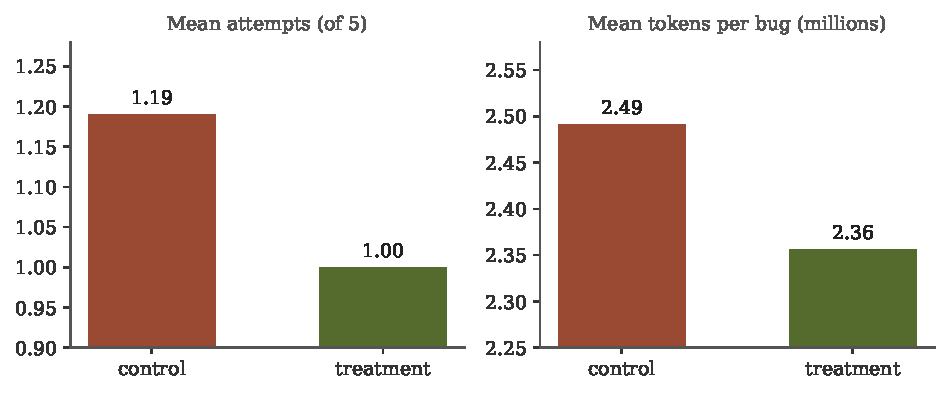
\includegraphics[width=\linewidth]{effort.pdf}
\caption{Effort per bug, matched pairs ($n{=}26$): mean attempts (of five allowed)
and mean tokens per bug. Treatment is lower on both, but the token gap is not a
uniform per-attempt saving---see below.}
\label{fig:effort}
\end{figure}

Splitting the 26 pairs by whether either arm needed a retry reframes the mechanism.
On the 22 bugs both arms solved in a \emph{single} attempt, the two arms are within
$\approx 3\%$ of each other in aggregate tokens (control $\approx 56.1$M vs.\
treatment $\approx 54.4$M)---close to a coin flip, with large bug-to-bug swings in
\emph{both} directions that nearly cancel. The entire net saving comes from four
bugs (\texttt{448702064}, \texttt{472538295}, \texttt{472567524},
\texttt{473582282}) where control needed extra attempts and treatment did not;
treatment did not require a retry on any matched bug (its mean attempt count is
exactly $1.00$). We therefore read the mechanism as: \emph{the playbook is not
making individual attempts cheaper; it is preventing some bugs from needing a
retry at all}---closer to pattern-matching a known bug family than to generally
sharper reasoning.

\subsection{The advantage tracks specific shapes, not the commonest one}

Grouping the solved bugs by root-cause tags (taken from the playbook's own tags,
not assigned by hand) gives a heavily skewed distribution: of 27 solved bugs, 10
share a single bigint stack/pool-lifetime pattern (use-after-return / pool
escape), 6 are MSan uninitialized-value bugs, and the rest fall into smaller
families (bignum boxing type confusion, bigint Karatsuba scratch-buffer overflow,
GC write-barrier/arena lifetime, and one-offs).

If the playbook helped most where it had the most examples, the retry-avoidance
would appear in that dominant family. It does not (Table~\ref{tab:family}). The
most repeated family needed \emph{zero} control retries and cost slightly
\emph{more} under treatment; every retry-avoidance bug sits in one of the smaller
families instead. The advantage tracks specific bug shapes the playbook happens to
have seen before, not the single most common shape.

\begin{table}[h]
\centering
\small
\begin{tabular}{lcccc}
\toprule
Family & $n$ & Ctrl att. & Trt att. & Token diff \\
\midrule
bigint stack/pool lifetime    & 9 & 1.00 & 1.00 & $+13.8\%$ \\
MSan uninitialized value      & 6 & 1.17 & 1.00 & $-44.5\%$ \\
other / one-off               & 4 & 1.00 & 1.00 & $-25.8\%$ \\
bignum boxing type confusion  & 3 & 1.33 & 1.00 & $+22.4\%$ \\
GC write-barrier / arena      & 2 & 1.50 & 1.00 & $-11.3\%$ \\
bigint Karatsuba scratch-buf. & 2 & 2.00 & 1.00 & $+6.6\%$ \\
\bottomrule
\end{tabular}
\caption{Per-family effort (matched pairs, $n{=}26$). ``Token diff'' is treatment
relative to control. The dominant family (top row) shows no control retries and a
small treatment \emph{penalty}; the retry-avoidance is in the smaller families.}
\label{tab:family}
\end{table}

\begin{figure}[h]
\centering
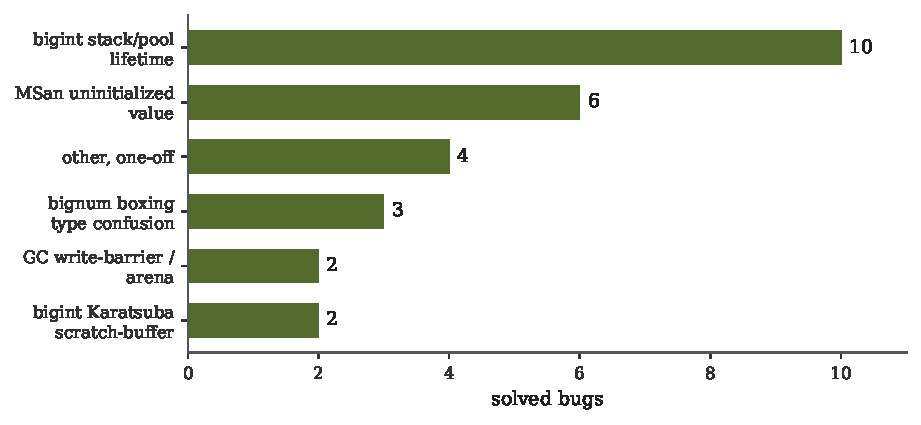
\includegraphics[width=\linewidth]{families.pdf}
\caption{Root-cause family distribution of the 27 solved bugs. Over a third share a
single bigint stack/pool-lifetime pattern, yet the retry-avoidance effect falls in
the \emph{smaller} families (Table~\ref{tab:family}).}
\label{fig:families}
\end{figure}

\section{What ``Needed a Retry'' Actually Conflates}
\label{sec:retry}

Because the entire measurable effect rides on a handful of control retries, we read
the archived per-attempt transcripts for those bugs. ``Needed a retry'' turns out
to bundle several very different causes that a single attempt-count field cannot
distinguish:
\begin{itemize}
  \item a genuine model \emph{safeguard refusal} on an ordinary, benign action,
  confirmed directly in two control transcripts;
  \item an apparent container out-of-memory kill (exit code 137) mid-verification,
  \emph{after} the agent had already root-caused the bug and built a working-looking
  fix;
  \item run-to-run \emph{nondeterminism}: two bugs each took multiple attempts on
  one run and a single attempt on an identical rerun;
  \item a real \emph{pipeline bug} (since fixed): the repair loop discarded an
  entire attempt---including a correct, working diff---whenever a usage-limit
  signal arrived, before checking whether a patch had been produced. This affected
  two bugs whose fixes would otherwise have been recorded on the first attempt.
\end{itemize}
None of this has been done systematically across every retry (it is manual
transcript reading, not an automated classifier), so the efficiency numbers in
Section~\ref{sec:results} should be read as \emph{not yet corrected} for
refusal- and infrastructure-driven retries. Because those causes fall on the
control arm here, correcting for them would tend to \emph{shrink} the apparent
treatment advantage; we cannot currently bound by how much.

\section{Running the Same Pipeline on a Local Model}
\label{sec:local}

Everything above uses a frontier, metered model as the repair agent. A separate,
exploratory question is whether the \emph{same} pipeline---holdout-safe playbook,
independent verification, differential oracle---can run on a small model served
locally, for the routine bugs. This section reports that extension; its numbers
are not directly comparable to the main experiment (single attempt per bug rather
than five, a different agent model), and are best read as a capability sketch.

\paragraph{Two harness bugs came first.} Swapping the agent model surfaced two
defects in our own harness that had been masked as model failures. (i)~The
recon-to-edit forcing gate counted \emph{any} file edit, so stray edits to a
scratch copy of the source satisfied it while nothing submittable had been written;
we scoped the count to the tree a patch is actually submitted from. (ii)~The
in-turn self-check reused a single warm build container and never reset its source
tree between checks, so the first diff that applied left the tree dirty and every
later diff failed to apply; resetting to a pristine tree before each apply, plus a
three-way apply, took the ``did not apply'' failure from the dominant self-check
outcome to zero on a bug that had previously been stuck on it. Fixing these moved
the wall from diff \emph{plumbing} to fix \emph{correctness}.

\paragraph{A higher-benchmark model that could not drive the loop.} Our first
replacement candidate scored higher than the incumbent on public coding
benchmarks. In this agentic harness it never completed the edit-then-check loop:
across four runs and three successive mitigations it looped on ``meta'' tools
(asking a nonexistent user, task-management, re-reading the source) and never
committed an edit. Its stated reasoning was on target; it could not \emph{execute}
the loop, and we reverted. We take this as a concrete instance of a general
caution: a benchmark score need not predict agentic harness fit.

\paragraph{What the small model solves.} The retained 24B open-weight model, at a
single attempt per bug over 20 bugs, produced 12 \texttt{verified\_correct} fixes
(60\,\%), each independently \texttt{oracle\_confirmed}. Broken out by bug family
(Table~\ref{tab:local}), it cleanly handles the routine, recurring families and
hits a bounded correctness ceiling on the subtlest root causes---uninitialized-value
and use-after-free---where it produces applying, compiling patches that do not
actually fix the bug. This is a characterizable frontier, not a blanket
incapacity, and it was obtained at a single attempt where the main experiment
allowed five.

\begin{table}[h]
\centering
\small
\begin{tabular}{lc}
\toprule
Bug family & Solved / seen \\
\midrule
Stack use-after-return (pool/stack escape) & 4 / 4 \\
Invalid-free                               & 1 / 1 \\
Stack-buffer-overflow                      & 1 / 1 \\
Segfault                                   & 2 / 3 \\
Heap-buffer-overflow                       & 2 / 4 \\
MSan uninitialized value                   & 2 / 6 \\
Heap use-after-free                        & 0 / 1 \\
\bottomrule
\end{tabular}
\caption{Local 24B model, single attempt per bug: 12/20 solved, all
\texttt{oracle\_confirmed}.}
\label{tab:local}
\end{table}

\begin{figure}[h]
\centering
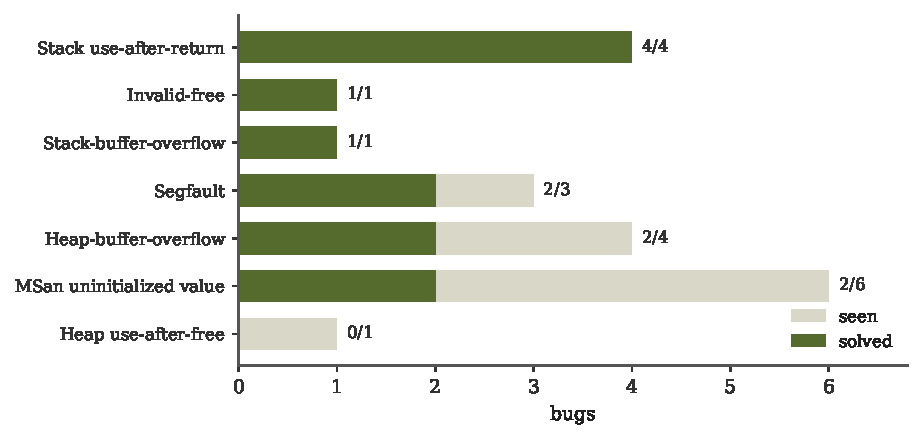
\includegraphics[width=\linewidth]{local.pdf}
\caption{Local 24B model, single attempt per bug: solved vs.\ seen by family (all
solves \texttt{oracle\_confirmed}). Routine families are handled cleanly; the
ceiling is on uninitialized-value and use-after-free.}
\label{fig:local}
\end{figure}

\section{Threats to Validity}
\label{sec:threats}

\textbf{Sample size and ceiling.} $N=30$ (27 runnable) is pilot scale, and both
arms are at a 100\,\% fix rate, so any control/treatment delta is directional
signal, not statistical proof; we report no significance tests because the design
does not support them. \textbf{Uncorrected confounds.} As Section~\ref{sec:retry}
details, the efficiency gap is not yet corrected for refusal-, OOM-, and
nondeterminism-driven retries, all of which happen to fall on the control arm in
this snapshot. \textbf{Nondeterminism.} At least two bugs changed attempt count
between identical reruns, so single-run per-bug efficiency figures carry real
run-to-run variance. \textbf{Oracle semantics.} \texttt{oracle\_confirmed} means
agreement with the upstream fix's behavior on the PoC and six probes, not absolute
correctness. \textbf{Single project.} All bugs are from mruby; we make no claim
about cross-project transfer. \textbf{Incomplete snapshot.} One control bug is
still rerunning and the local-model control arm is not included here; both are
excluded rather than estimated.

\section{Conclusion}

On this pilot the injected playbook does not change \emph{whether} an mruby bug
gets fixed---both arms fix everything they complete---and its measurable effect on
effort is small ($\approx 5\%$ fewer tokens, $1.19\!\rightarrow\!1.00$
attempts). More informative than the magnitude is the \emph{shape} of the effect:
it is not a uniform per-attempt saving but the avoidance of a few specific retries,
concentrated on bug families the playbook had already seen, and even that signal is
entangled with refusals and infrastructure noise we have only begun to separate.
The most defensible reading is that, at this scale, a learned playbook behaves more
like recognition of a previously seen bug shape than like generally improved
reasoning. The infrastructure built here---holdout-safe injection, deployment-faithful
verification, and a differential oracle---is what would be needed to test that
reading at a larger scale, and, as the local-model extension suggests, to do so on
cheaper inference for the routine cases.

\paragraph{Reproducibility.} The dataset is public (ARVO); the exact protocol,
per-bug ledger, and commands are in the accompanying repository.

\begin{thebibliography}{9}
\bibitem{arvo} ARVO: Atlas of Reproducible Vulnerabilities for Open Source
software. \url{https://github.com/n132/ARVO}.
\bibitem{ossfuzz} OSS-Fuzz: continuous fuzzing for open source software.
\url{https://github.com/google/oss-fuzz}.
\bibitem{mruby} mruby: lightweight implementation of the Ruby language.
\url{https://github.com/mruby/mruby}.
\end{thebibliography}

\end{document}
